\section{Porównanie działania algorytmów}
Testy algorytmów zostały przeprowadzone na grupie 10 instancji testowych o różnym rozmiarze: od 33 do 403 miast. Na każdej z instancji każdy z algorytmów został uruchomiony dziesięciokrotnie w celu ustalenia zarówno wartości średniej jak i rozproszenia poszczególnych mierzonych parametrów. Testy przeprowadzono na maszynie wyposażonej w procesor Intel Core i7-620M oraz 4GB pamięci RAM. 

Zaimplementowane algorytmy to algorytm losowy oraz algorytmy przeszukiwania lokalnego -- Greedy, Steepest, Tabu Search oraz Simulated Annealing. Przygotowana została także prosta heurystyka w celu porównania uzyskanych wyników. W jej formie użyto algorytmu zachłannego, który po wylosowaniu punktu startowego przechodzi do najbliższego z sąsiadujących miast, które nie zostało jeszcze odwiedzone.

Wyniki zostaną obecnie zaprezentowane w poszczególnych punktach.

\subsection{Jakość działania}
Optymalne wartości funkcji celu dla każdej instancji były znane a priori, dlatego też jako miarę jakości działania algorytmów wykorzystano następującą zależność:
\begin{equation*}
fitness = \frac{f_{alg}(\Pi_i)}{f_{OPT}(\Pi_i)}*100\%
\end{equation*}
gdzie:

\begin{table}[h!]
       \begin{tabular}{lll}
       	$fitness$ & --- & jakość algorytmu\\ 
        $f_{alg}(\Pi_{i})$ & --- & wartość funkcji celu rozwiązania zwracanego przez badany \\
        &&algorytm dla instancji $\Pi_i$\\ 
		$f_{OPT}(\Pi_{i})$ & --- & wartość funkcji celu rozwiązania optymalnego dla instancji $\Pi_i$
		\end{tabular}
\end{table}
\noindent Jeżeli algorytm zwróci rozwiązanie optymalne, miara jakości wyniesie 100\%. Wraz z pogarszaniem się zwracanego wyniku miara jakości będzie rosła, wyznaczając stosunkowy stopień oddalenia od wartości optymalnej.

\begin{figure}[!h]
\centering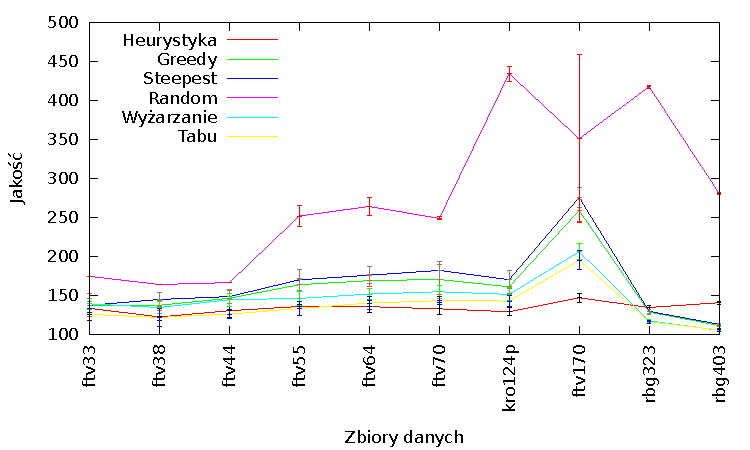
\includegraphics[width=12cm]{img/jakosc_avg}
\caption{Jakość działania poszczególnych algorytmów dla przypadku średniego.}\label{rys:jakosc_avg}
\end{figure}

\begin{figure}[!h]
\centering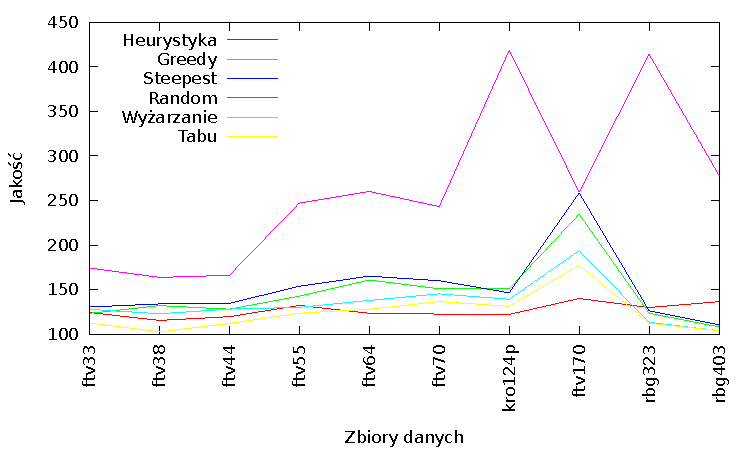
\includegraphics[width=12cm]{img/jakosc_best}
\caption{Jakość działania poszczególnych algorytmów dla przypadku najlepszego.}\label{rys:jakosc_best}
\end{figure}

Rysunki \ref{rys:jakosc_avg} oraz \ref{rys:jakosc_best} przedstawiają wyniki testów jakości odpowiednio dla przypadku średniego i najlepszego. Najlepsze wyniki zostają zwracane przez heurystykę. Jakość działania algorytmów przeszukiwania lokalnego jest bardzo zbliżona. Najgorzej wypada algorytm losowy -- przy mniejszych instancjach zwracane przez niego wyniki nie odbiegają jeszcze tak bardzo jakościowo od pozostałych algorytmów, wraz z liniowym wzrostem rozmiaru instancji rozmiar przestrzeni rozwiązań dopuszczalnych rośnie jednak wykładniczo, przez co proste strzelanie w wynik staje się dużo mniej opłacalne. Spośród algorytmów przeszukiwania lokalnego najlepiej wypada Tabu Search, a następnie Simulated Annealing. Jednak o ile pierwszy z tych algorytmów jest bardziej zbliżony pod względem jakości do heurystyki, o tyle drugi z nich działa podobnie do algorytmów Greedy i Steepest.

Jeżeli chodzi o rozproszenie jakości zwracanych rozwiązań, wyniki zwracane przez heurystykę są bardzo zbliżone. Algorytmy przeszukiwania lokalnego zwracają wyniki nieznacznie bardziej rozrzucone wokół wartości średniej. Algorytm losowy zachowuje się natomiast całkowicie losowo -- widzimy tu przypadki od praktycznie zerowego rozrzucenia, przez to porównywalne do algorytmów lokalnych, kończąc na kilkukrotnie od nich wyższym.

Porównując wykresy dla przypadku średniego i najlepszego zauważyć można wyraźnie, że tendencja jest zachowana, jedynie wykresy znajdują się o kilka punktów procentowych niżej.

\subsection{Czas}
Do pomiaru czasu skorzystano z timera udostępnionego razem z biblioteką \emph{boost}. Zwraca on wynik w postaci wartości podwójnej precyzji (\texttt{double}), rozpoczynając od $0,001$s. W celu dokładniejszego wyznaczenia czasu wywołań algorytmów dla najmniejszych instancji, powtarzano uruchamianie z tego samego punktu startowego minimalnie przez $0,5$s, po czym otrzymany czas dzielono przez liczbę wykonań algorytmu.

\begin{figure}[!h]
\centering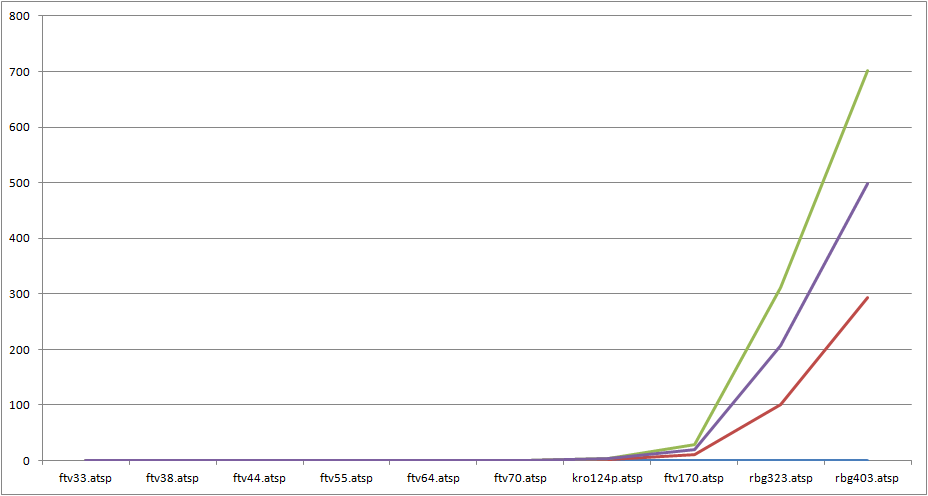
\includegraphics[width=12cm]{img/czas_avg}
\caption{Czas działania poszczególnych algorytmów dla przypadku średniego.}\label{rys:czas_avg}
\end{figure}

Rysunek \ref{rys:czas_avg} przedstawia wyniki badania czasu działania poszczególnych algorytmów dla przypadku średniego. Ponownie, najlepiej spisała się heurytyka, która posiada złożoność $O(n^2)$, co nawet dla największej badanej instancji daje wynik nieprzekraczający $0,01$s (na wykresie linia odpowiadająca heurystyce pokrywa się z osią odciętych, przez co jest praktycznie niewidoczna). Na drugim miejscu znalazł się algorytm Simulated Annealing. Problemem w ocenie efektywności czasowej tego algorytmu jest dobór parametrów, które w znaczący sposób wpływają na czas jego działania. Algorytmy Greedy oraz Tabu Search działają w podobnym czasie, co dla tego pierwszego wynika z tego, że szybciej niż algorytm Steepest odwiedza on kolejnych sąsiadów. W przypadku Tabu Search dla dużej instancji -- 403 miasta -- działał w czasie krószym niż Greedy, co z kolei może oznaczać, że przez dodatkowe warunki działania algorytmu odwiedza on mniejszą liczbę sąsiadów, chociaż nie ma to wpływu na jakość jego działania. Steepest spisał się najgorzej, gdyż przed przejściem do kolejnego sąsiada musi przejrzeć wszystkich swoich sąsiadów ($\frac{n(n-1)}{2}$).

Algorytm losowy nie kończy się w sposób naturalny. W celu zachowania równych szans, czas po którym algorytm był zatrzymywany został określony na poziomie średniej arytmetycznej czasu działania algorytmów Greedy i Steepest. Jako że czas działania został ustalony w sposób sztuczny, analizowanie go byłoby bezpodstawne.

\subsection{Współczynnik czas/jakość}
Wybierając algorytm nie zawsze interesuje nas to, by algorytm zwracał za wszelką cenę rozwiązanie jak najbardziej zbliżone do optymalnego. Czasami jesteśmy skłonni poświęcić odrobinę jakości kosztem krótszego czasu działania, szczególnie w systemach czasu rzeczywistego. Dlatego też konieczne jest wyznaczenie wartości, która uwzględniałaby oba te czynniki naraz.

Jako pierwszy krok, z wyników przeprowadzonych testów (również na innych instancjach niż te omawiane w poniższym sprawozdaniu) wybrano najlepsze i najgorsze wartości dla czasu i jakości. Wyniosły one odpowiednio $0,001$s i $754,89$s oraz $100\%$ i $542,76\%$. Następnie, średnie wyniki czasu działania i jakości badanych algorytmów znormalizowano do wartości z przedziału $<0,1>$ -- $0$ dla rozwiązania najgorszego, $1$ dla najlepszego. Korzystając z tych znormalizowanych wartości przystąpiono do wyznaczenia współczynnika cena/jakość zgodnie ze wzorem na ważoną średnią harmoniczną:
\begin{equation*}
price\_fitness = \frac{2}{\frac{1}{time_{norm} + \epsilon} + \frac{1}{fitness_{norm} + \epsilon} }
\end{equation*}

Do wartości znormalizowanych współczynników czasu i jakości dodajemy nieskończenie małą wartość $\epsilon$ w celu uniknięcia dzielenia przez 0. Wówczas jeśli którykolwiek z tych współczynników wyniesie $0$ dla danego algorytmu, to we wzorze na współczynnik ceny do jakości uzyskamy $\frac{2}{\frac{1}{time_{norm} + \epsilon} + \frac{1}{0 + \epsilon}}$, co oznacza, że mamy $\frac{2}{1 + \infty}$, czyli ostatecznie $0$.

 Okazuje się, że tak zdefiniowany współczynniki czasu do jakości umożliwia dobrą klasyfikację algorytmów ze względu na ich badane cechy. Algorytm działający w najkrótszym czasie, zwracający najlepszy wynik, otrzyma współczynnik cena/jakość równy $1$, najgorszy -- $0$. Słaba wartość któregokolwiek ze znormalizowanych czynników natychmiast obniża wartość współczynnika. Jednak przykładowo algorytm zwracający najlepsze rozwiązania, ale działający najwolniej otrzyma wartość współczynnika równą 0.

\begin{figure}[!h]
\centering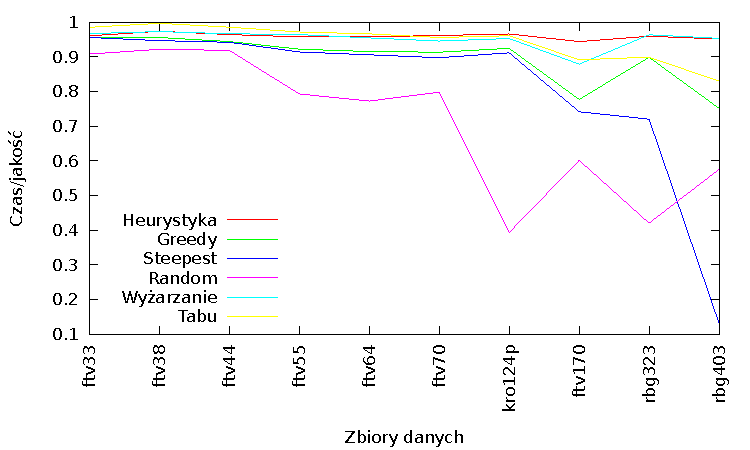
\includegraphics[width=12cm]{img/jakosc-czas}
\caption{Współczynnik czas/jakość dla poszczególnych instancji i poszczególnych algorytmów dla przypadku średniego.}\label{rys:czas_jakosc}
\end{figure}

Jako, że heurystyka spisała się najlepiej zarówno pod względem czasu jak i jakości zwracanych wyników, jej współczynnik czas/jakość niemalże sięga wartości $1$. Trochę zaskakujący może być fakt, że algorytmy Tabu Search oraz Simulated Annealing, które są w zasadzie modyfikacjami algorytmów Greedy/Steepest, osiągnęły również bardzo wysoki współczynniki czasu do jakości. Ma to jednak uzasadnienie w sposobie działania tych algorytmów -- o ile Greedy i Steepest bardzo łatwo wpadają w minima lokalne, o tyle Tabu Search oraz Simulated Annealing posiadają mechanizmy, które umożliwiają im wyskoczenie z takich minimów lokalnych poprzez wybranie ruchu pogarszającego obecne rozwiązanie. Dzięki temu potrafią przejrzeć większe spektrum rozwiązań i mogą zbadać kilka minimów lokalnych w ramach jednego uruchomienia i wybrać najlepsze z nich. Na kolejnym miejscu znalazł się algorytm Greedy, który wygrał z algorytmem Steepest głównie na gruncie czasu działania. Algorytm losowy po raz kolejny zachowuje się nieprzewidywalnie, wraz ze wzrostem rozmiaru instancji wartość jego współczynnika czas/jakość spada, głównie za sprawą zdecydowanego spadku w jakości zwracanych rozwiązań.

\subsection{Średnia liczba kroków oraz ocenionych rozwiązań algorytmów przeszukiwania lokalnego}
Algorytmy Steepest i Greedy działają w odmienny sposób. Steepest, zanim przejdzie do któregoś z sąsiadów, przegląda wszystkich swoich sąsiadów w celu znalezienia tego najlepszego. Greedy natomiast po trafieniu na pierwszego lepszego od siebie sąsiada natychmiast do niego przechodzi. Oznacza to, że Steepest powinien docierać do wyniku w mniejszej liczbie kroków (każdy krok wiąże się z wyższą różnicą funkcji celu), jednak przeglądając większą liczbę rozwiązań.

Z kolei algorytmy Tabu Search oraz Simulated Annealing działają w nieco inny sposób. W przypadku tego pierwszego generowany jest podzbiór sąsiedztwa o mocy potrojonej długość instancji, którego elementy następnie zostają poddane rankingowi. Wybierany jest najlepszy z ruchów, ale lista pozostałych ruchów nie jest unieważniania -- tworzy tzw. listę elitarnych kandydatów. W kolejnej iteracji ruchy znajdujące się na tej liście są ponownie reewaluowane (przeliczana jest funkcja celu rozwiązania uzyskanego przez wykonanie danego ruchu) i wybierany jest kolejny ruch. Proces ten jest powtarzany do momentu aż najlepszy z ruchów na tej liście okaże się być gorszym (pod względem poprawy wartości funkcji celu) od najgorszego z listy początkowej (z której wygenerowano listę elitarnych kandydatów). Wówczas ponownie generowany jest podzbiór sąsiadów i proces jest powtarzany od początku. Ponadto dany ruch może być zabroniony ze względu na bycie ,,tabu'' i wówczas nie może zostać wykonany jeśli nie zostaną spełnione pewne specjalne kryteria aspiracji (np. poprawienie funkcji celu w taki sposób, że będzie lepsza niż dotychczas znaleziona wartość minimalna). W związku z tym spodziewamy się, że algorytm ten przejrzy znacznie mniejszą liczbę sąsiadów.

Simulated Annealing posiada trochę inny mechanizm przechodzenia do sąsiadów w porównaniu do pozostałych algorytmów przeszukiwania lokalnego. Startuje on z pewnym poziomem temperatury, która ma wpływ na prawdopodobieństwo przeskoczenia do danego sąsiada. Wartość początkowa temperatury wyznaczana jest w oparciu o średnią różnicę funkcji celu wewnątrz sąsiedztwa -- jendokrotnie przeglądane jest całe sąsiedztwo punktu startowego w celu wyznaczenia tej wartości, po czym jako temperaturę startową przyjmowana jest jej czwarta część. Wartość ta jest wystarczająca by zaakceptować nawet zdecydowanie gorszych sąsiadów. W trakcie działania algorytmu temperatura powoli jest obniżana, co zmniejsza szanse wykonania skoku. Sposób obniżania temperatury jest parametrem algorytmu -- dla naszego przypadku przyjęliśmy, że obniżamy ją w sposób procentowy (80\% poprzedniej wartości) co pewną liczbę przejrzanych sąsiadów (równą liczności jednego sąsiedztwa) na danym jej poziomie. W związku z tym wydaje się, że algorytm wykona większą liczbę kroków, ale przejrzy mniejszą liczbę sąsiadów z powodu przedstawionej procedury. Można więc przyrównać działanie tego algorytmu do działania algorytmu Greedy -- w tym wypadku skok nie następuje do lepszego rozwiązania, tylko wynika z funkcji prawdopodobieństwa zależnej od temperatury. Z powodu kilku iteracji procesu obniżania tej temperatury algorytm wykonuje znacznie większą liczbę kroków, mimo przeglądania małej liczby sąsiadów. Należy zaznaczyć, że dzięki funkcji prawdopodobieństwa dla wykonania skoku algorytm ten może przejść do rozwiązania gorszego -- wraz ze zmniejszaniem się wartości temperatury prawdopodobieństwo to jednak maleje.

\begin{figure}[!h]
\centering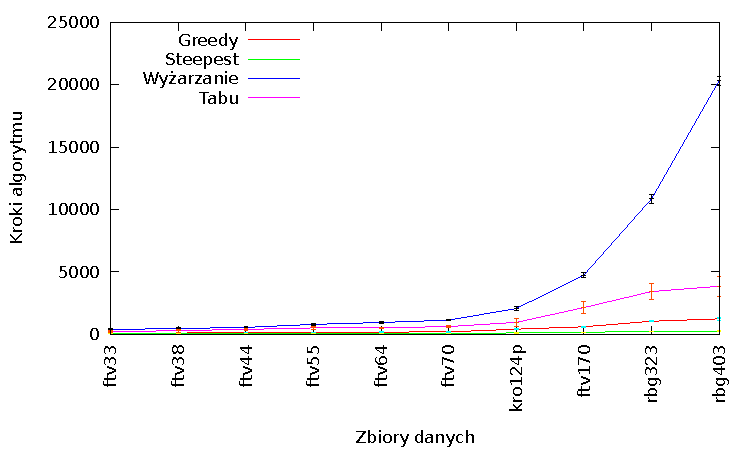
\includegraphics[width=12cm]{img/loc_skoki}
\caption{Średnia liczba kroków w dojściu do optimum lokalnego.}\label{rys:loc_skoki}
\end{figure}

\begin{figure}[!h]
\centering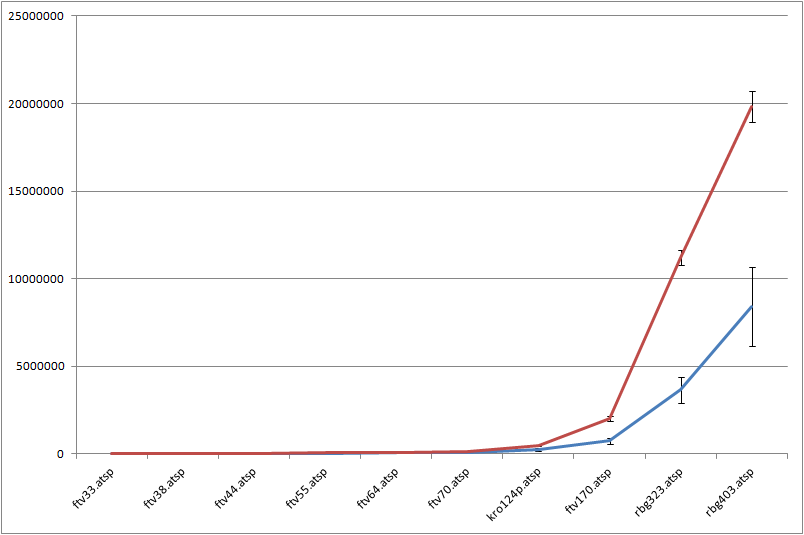
\includegraphics[width=12cm]{img/loc_sasiedzi}
\caption{Średnia liczba przejrzanych rozwiązań w dojściu do optimum lokalnego.}\label{rys:loc_sasiedzi}
\end{figure}

Rysunki \ref{rys:loc_skoki} i \ref{rys:loc_sasiedzi} potwierdzają przedstawione wcześniej tezy. Algorytm Greedy faktycznie dochodzi do lokalnego optimum wykonując więcej mniejszych skoków, natomiast algorytm Steepest przegląda większą liczbę rozwiązań sąsiednich. Simulated Annealing przegląda najmniejszą liczbę sąsiadów, ale wykonuje najwięcej iteracji. Z kolei Tabu Search wykonuje sporo dodatkowych kroków, ale przegląda mniejszą liczbę sąsiadów niż algorytmy Greedy i Steepest.